\section{Experiments}
\label{sec:exp}

The experiments follow a mission similar to the original plan given in
Fig. \ref{fig:ex:plan}. The AUV needs to {\em Sample Vent2} and return
to the {\em surface} by the end of the mission. The AUV must also be
at the {\em surface} around
13:00. % with plans being produced by the europa planning engine
% \cite{frank2003}.
Fig. \ref{fig:ex:mixed1} demonstrates the resulting plan after being
processed by Algorithm \ref{alg:dispatch} using our executive \rx
which synthesizes temporal plans. We have also defined the policy
of earliest start time to the goals in plan.

\begin{figure}[!htbp]
  \centering
  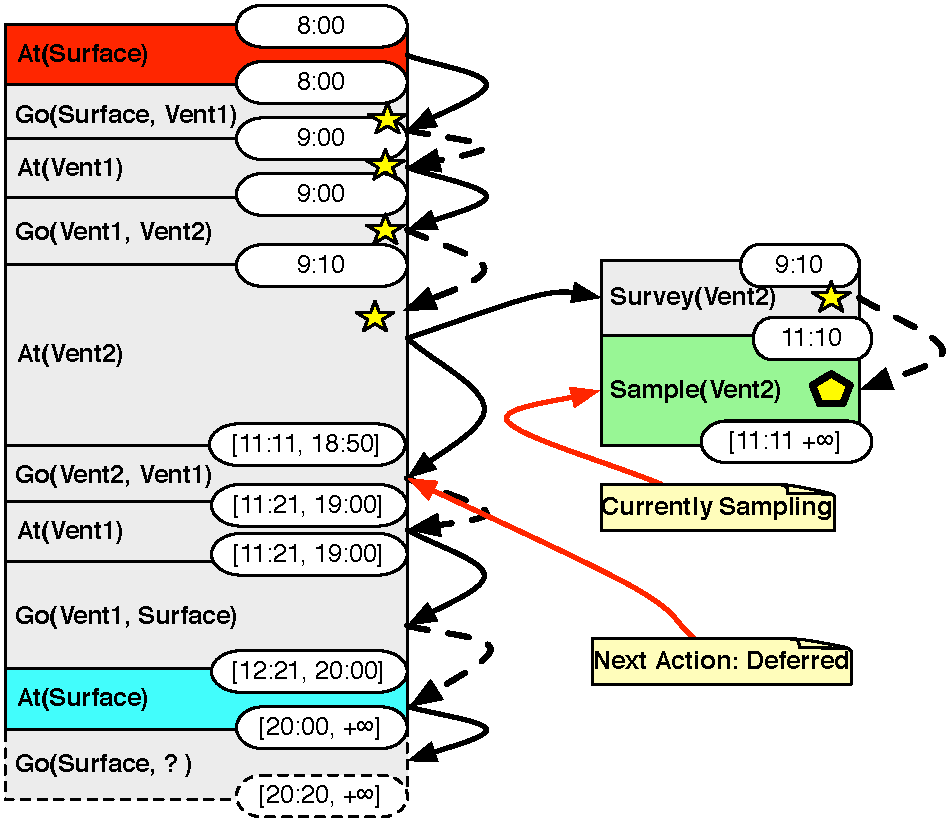
\includegraphics[width=0.9\columnwidth]{figs/example_MixedInitial}
  \vskip-2mm
  \caption{\small Solid lines indicate conditions and dashed lines
    indicate effects. Pentagons indicate {\em urgent} goals and stars
    indicate tokens that were deduced as {\em proactive}.}
  \label{fig:ex:mixed1}
  \vskip-3mm
\end{figure}

% For Algorithm \ref{SearchForGoal}, the search is straight forward. For
% example in 

% As shown in Fig. \ref{fig:ex:mixed1}, if the AUV is {\em At Surface}
% at execution time, the next {\em Go} token will be dispatched. Because
% the search follows causal links, it will encounter the {\em Sample
%   Vent2} goal resulting in dispatching proactively.  Similarly, this occurs
% for all of the tokens that are starred. The next token that is not
% starred, {\em Go(Surface)}, is continuously searched but deferred,
% because it is not connected to an urgent goal. The resulting AUV stays
% at {\em Vent2} rather than heading to the {\em Surface} immediately.

As in Fig. \ref{fig:ex:mixed1}, the AUV is {\em At Surface} initially.
At execution time, the next {\em Go} token will be dispatched
early, because when the search follows causal links, it
encounters the {\em Sample Vent2} goal.  This occurs similarly
for all tokens that are starred. {\em Go(Surface)} gets deferred,
because it is not connected to a goal using the forward
search. Consequently, the resulting execution requires the AUV to stay at {\em
  Vent2} rather than heading to the {\em Surface} immediately.

%For the distributed algorithm approach, each token is checked during
%the creation of the plan to see if it is an external goal in
%$\Phi_{ge}$, or connected to one through a causal link. When the {\em
%Sample Vent2} is checked, we immediately find that it is a goal. We then
%follow the reverse causal link and find {\em Survey Vent2}.  However to
%better illustrate the algorithm, we can imagine that only the {\em Survey
%Vent2} has been causally connected to the goal so far. Therefore, we
%only star those two tokens. The path from {\em Surface} to {\em Vent1}
%to {\em Vent2} has yet to be built. When the path has finally been
%built, and {\em At Vent2} is checked, our algorithm searches one
%causal link and finds {\em Survey Vent2} which is starred. The search
%then follows the reverse causal link and stars the rest of the
%path. The starred tokens will then be proactively dispatched while the
%non-starred tokens will be deferred until later. Having similar
%results to Algorithm \ref{DispatchToken}.

We then introduced a new goal to {\em Sample Vent1} at
11:30 with the resulting plan shown in Fig. \ref{fig:ex:mixed2}. Since
there is not enough time to {\em Sample Vent1} and be at the surface
by 13:00, the goal is placed after the AUV visits the
surface. Propagation results in marking the tokens, which were thus
far deferred and are now causally linked to the new
goal of {\em Sample Vent1}, as having the policy of the goal. The
resulting starred tokens get dispatched proactively which includes all
tokens related to the mid-day surfacing token.

\begin{figure}[t]
  \centering
  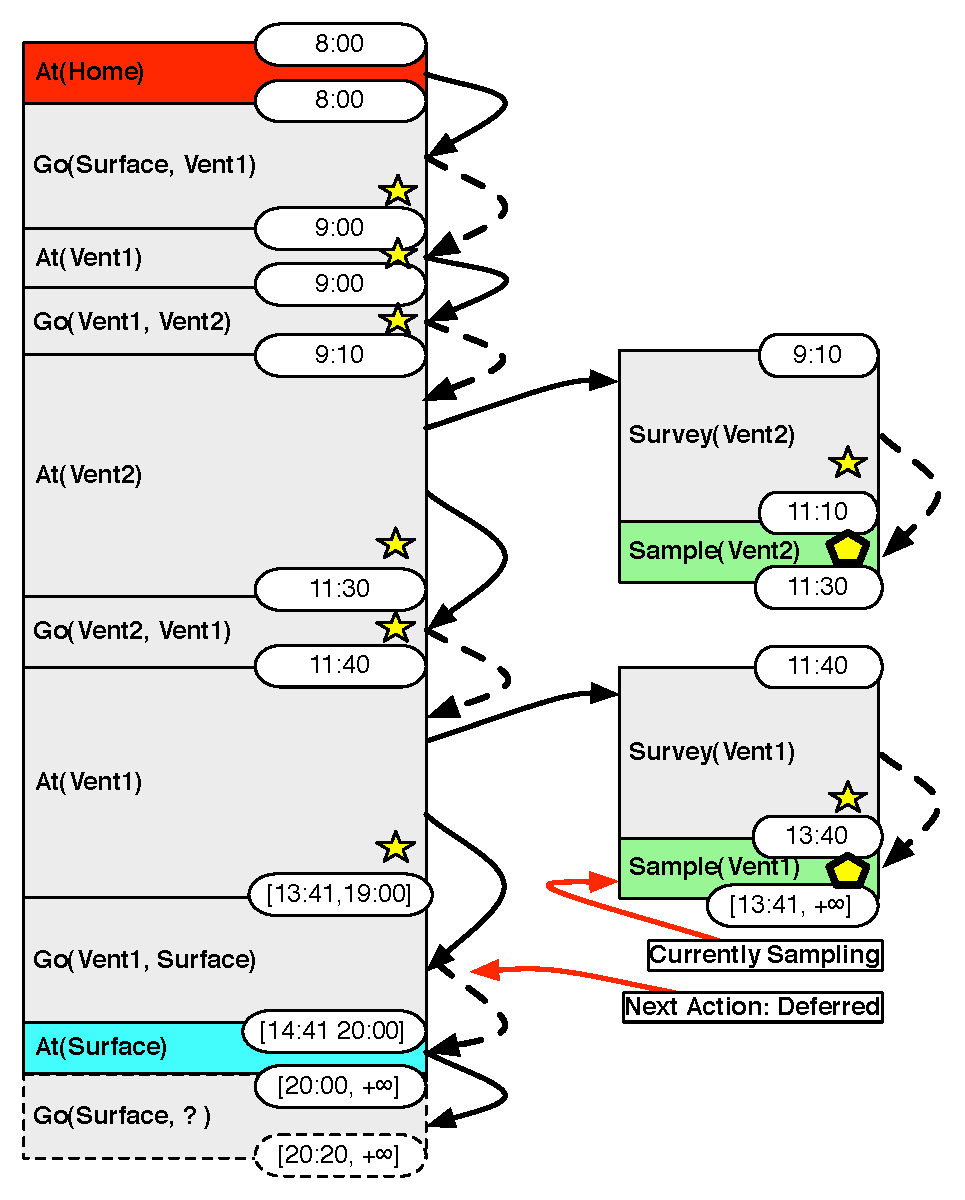
\includegraphics[width=0.8\columnwidth]{figs/example_MixedUpdate}
  \vskip-3mm
  \caption{\small The solution after receiving external request for
    the plan from Fig. \ref{fig:ex:mixed1}}
  \label{fig:ex:mixed2}
  \vskip-3mm
\end{figure}

Meanwhile, the tokens related to the final surfacing remain {\em
  deferred} and won't be executed until 19:00 allowing the vehicle to
sample {\em Vent1} for a duration of 2:50 hours.  After returning to
the {\em Surface}, our planner and domain inserted a partially
instantiated token to {\em Go(Surface, ?)} (dashed in the figures).
This is an artifact resulting from the plan model which specifies that
an {\em At} token is necessarily followed by a {\em Go}.  However, our
algorithm will not be dispatching this token as it is not connected to
a goal and its upper bound start time ($+\infty$) will
not be met within the scope of the mission.

\subsection{Performance Analysis}

In our experiments, the simulated AUV missions ran on a Linux virtual
machine running on a MacBook Pro allocated one core from a $2.33$ GHz
Intel Core $2$ Duo processor.
% Time was recorded using a thread clock for the most accurate time.
A short mission duration ($200$ seconds) was selected to allow rapid
assessment with multiple runs; increasing mission duration generates
no impact of significance.
% We chose a mission length of 200 seconds to allow simulation to
% be completed quickly. There is, however, no difference in performance
% if the mission were longer as the same plan would be produced just
% with different timepoints.
 
Fig. \ref{fig:example_run} shows a mission run that is similar to the
example in Fig. \ref{fig:ex:plan}.  To increase plan complexity a
total of $8$ intermediate locations were added between the {\em
  surface} and {\em vent 1}, with all evaluations taking less then $1$
millisecond. The largest performance spikes were due to the need to
evaluate the dispatching condition for an {\em At} token which is
followed by a {\em Go} token resulting in two forward searches within
the plan structure. This is because the dispatch window is larger than
the minimum duration of the {\em At} token; since our plan uses a {\em
  Go} immediately after, this \emph{Go} token also needs to be
evaluated.

\begin{figure*}[t]
  \centering
  \vskip-3mm
  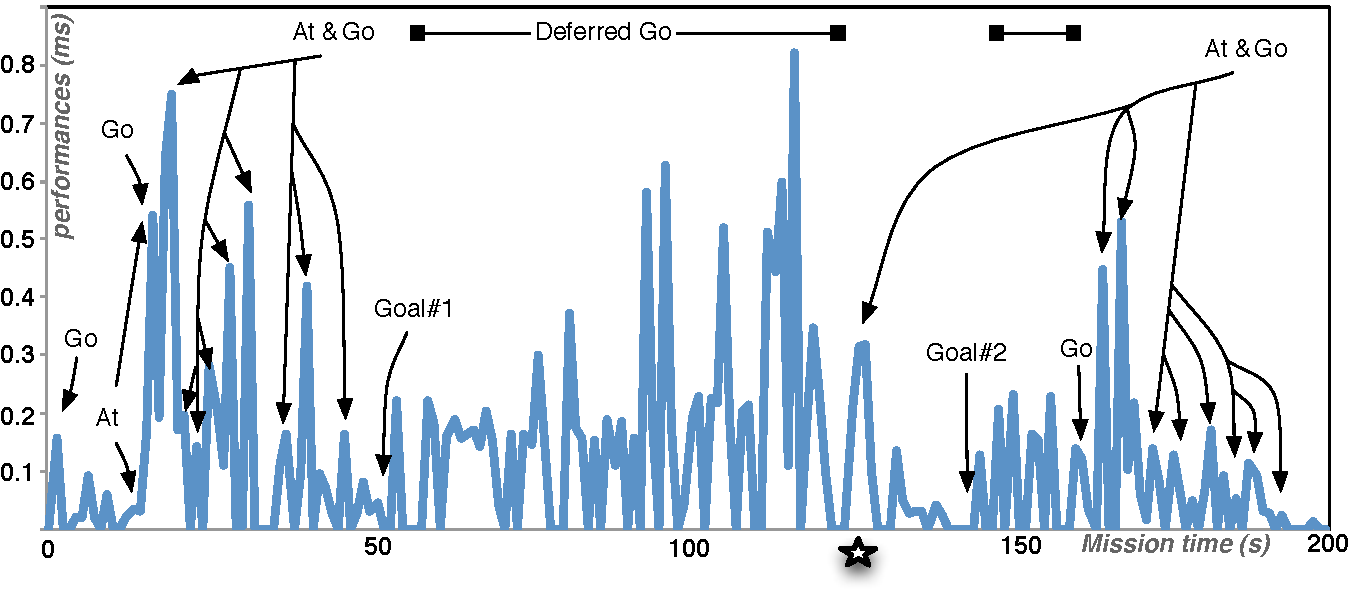
\includegraphics[width=1.2\columnwidth]{figs/example_run.pdf}
  \vskip-2mm
  \caption{\small A mission run that shows the time needed for
    dispatching. The star represents when Goal \#2 is received and
    integrated into the plan. Lines with boxes at the end represent
    the deferred action {\em Go} Because of space, we didn't put an
    arrow to every {\em At}. Our concern were the peaks that showed
    where the system had to dispatch both {\em At} and {\em Go}. }
  \label{fig:example_run}
  \vskip-2mm
\end{figure*}


We also identified a clear trend of a decrease in time as the agent
comes closer to the completion of either {\em Goal \#1} or {\em Goal
  \#2}. This is correlated to the reduction in search distance toward
these goals as we execute new tokens.  We see an important
variability in execution time which is likely due to context switching
between processes and threads within our agent; multiple cores in the
virtual machine is likely to remove this variation.  The bump in
timing between time-step $56$ and the introduction of {\em Goal \#2}
at $127$ is because the algorithm is continuously searching the graph
from the next {\em Go}, which during this period, is not connected to
a goal. The resulting exhaustive search in the plan
graph during this period is on an average above $0.2$ milliseconds. At
tick $127$, the {\em Go} is no longer deferred and gets dispatched.
% The search for our algorithm execution time {\em Goal \#2} becomes
% relatively simple as it is not very far away in the plan
% \kcomment{from what? from the end of the plan?}, and thus the time
% decreases significantly.

\begin{figure}[!b]
  \centering
  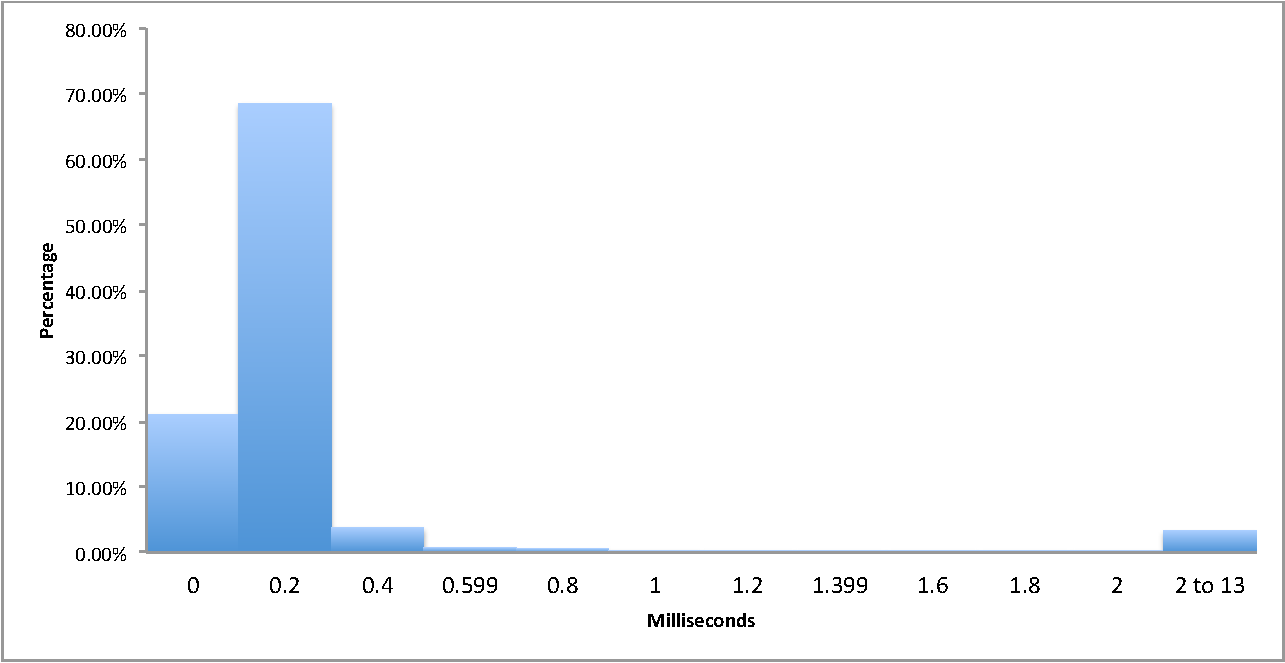
\includegraphics[width=\columnwidth]{figs/HistogramAlg1}
  \caption{\small Algorithm \ref{alg:dispatch} was timed at every
    increment ($1$ Hz) for $500$ simulated missions. One goal was
    inserted into the plan at random during the mission. The histogram
    shows the distribution of the time, which is heavily skewed to the
    left.}
  \label{fig:histogram}
\end{figure}

% In order to demonstrate the average amount of time that Algorithm
% \ref{DispatchToken} uses, $500$ simulated missions were recorded and
% timed at every increment of the mission time. 
Fig. \ref{fig:histogram} shows the distribution of execution time for
$500$ simulated missions. It shows that $90\%$ of the time our
algorithm completed its search in less than $0.2$ milliseconds. The
distribution is long tailed with the worst performance between $2$ and
$13ms$ occurring for less than $5\%$ of the runs. Such performance is
exhibited when the {\em tokens} evaluated are meant to be {\em
  deferred} which is not critical to the overall execution.

% which makes the small loss of performances not as
% critical.


%%% Local Variables: 
%%% mode: latex
%%% TeX-master: "aaai13"
%%% End: 
